\appendix
\clearpage
\pdfbookmark{Anhang}{anhang}

\addcontentsline{toc}{chapter}{Anhang}


\chapter{Model of Expert Performance}
\label{chap:ModelofExpert}

\begin{figure}[h]
    \centering
    \frame{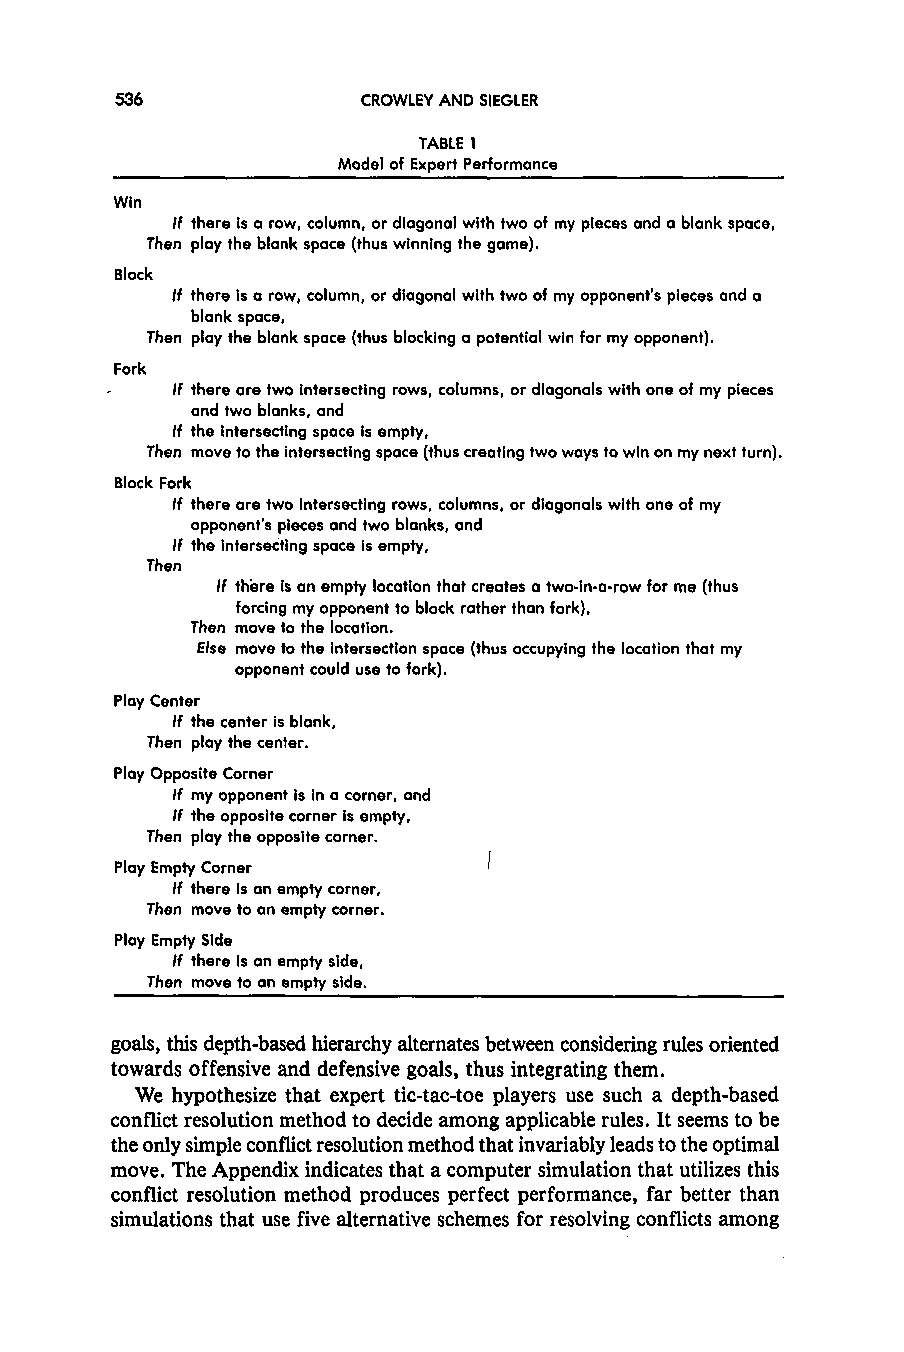
\includegraphics[width=0.7\linewidth]{04_Artefakte/crowley_expertplay.pdf}}
    \caption[Model of Expert Performance]{Model of Expert Performance von \citeauthor{crowleyFlexibleStrategyUse1993}, Auszug aus \cite[S. 536]{crowleyFlexibleStrategyUse1993}}
\end{figure}

\chapter{Beispiel für Meta-Log der Implementierung}
\label{chap:meta}
\begin{longlisting}
\caption{Meta-Log der Implementierung}
\label{listing:meta}
\inputminted{text}{04_Artefakte/03_Listings/meta.txt}
\end{longlisting}



\chapter{minimax-Methode}
\label{chap:minimax_listing}
\begin{longlisting}
\caption{minimax-Methode der Klasse MinimaxAlgorithm}
\label{listing:minimax}
\inputminted{java}{04_Artefakte/03_Listings/minimax.java}
\end{longlisting}



\chapter{Zusätzliche Auswertung zu Q-Learning}
\label{chap:app_qlearning}
\section{Konvergenz alternierendes Self-play}

\begin{figure}[h]
\centering
\begin{subfigure}[b]{0.75\textwidth}
    \centering
   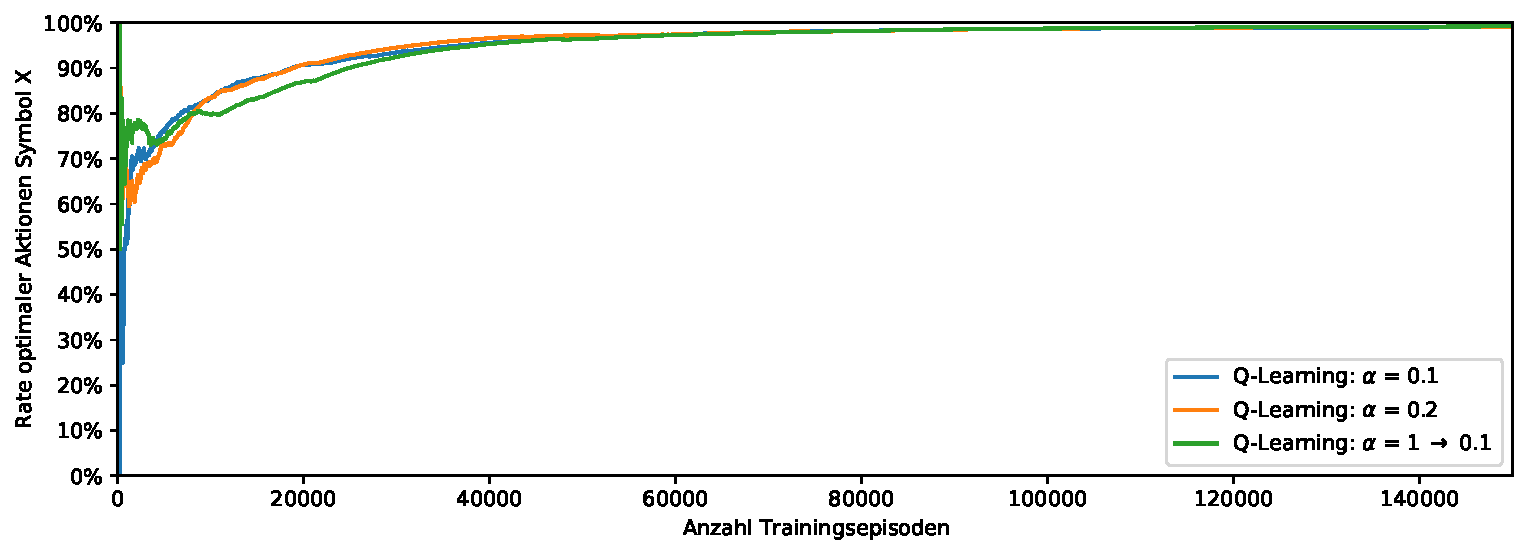
\includegraphics[width=1\linewidth]{convergence/convergence_compare_alpha_QLearning_ALTERNATE_X.pdf}
   \caption{Symbol X}
   \label{fig:convergence_compare_alpha_QLearning_ALTERNATE_X} 
\end{subfigure}

\begin{subfigure}[b]{0.75\textwidth}
    \centering
   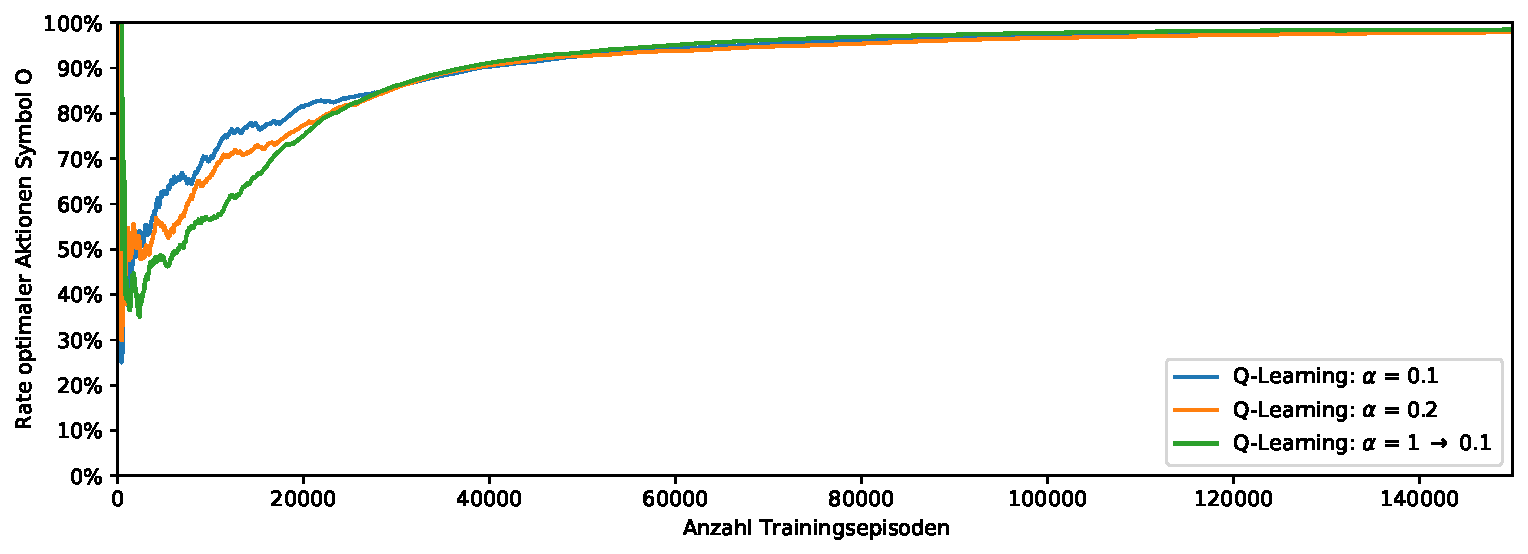
\includegraphics[width=1\linewidth]{convergence/convergence_compare_alpha_QLearning_ALTERNATE_O.pdf}
   \caption{Sybmol O}
   \label{fig:convergence_compare_alpha_QLearning_ALTERNATE_O}
\end{subfigure}
\caption[Rate optimaler Aktionen Q-Learning unterschiedliche Lernraten, alternierendes \splay]{Rate optimaler Aktionen von Q-Learning für verschiedene Lernraten $\alpha$, alternierendes \splay (a) Symbol X (b) Symbol O}
\label{fig:convergence_compare_alpha_QLearning_ALTERNATE}
\end{figure}

\section{Spielergebnismatritzen klassisches Self-play}
\begin{table}[ht]
\centering
\caption[Spielergebnismatrix \qlearning: $\alpha=0,2$, klassisches \splay]{Spielergebnismatrix für \qlearning mit Lernrate $\alpha=0,2$, klassisches \splay}
\label{tab:resultmatrix_ql_normal_alpha02}

\begin{tabular}{llrlr}
\toprule
 & \multicolumn{2}{l}{\textbf{Minimax}} & \multicolumn{2}{l}{\textbf{Random}} \\ \midrule
\textbf{X Q-Learning}   & X Q-Learning:     & 0,00\% $\pm$    0,00\%            & X Q-Learning:         & 98,91\% $\pm$ 0,31\%  \\
                        & O Minimax:        & 0,00\% $\pm$    0,00\%            & O Random:             & 0,00\% $\pm$  0,00\%  \\
                        & Unentschieden:    & 100,00\% $\pm$  0,00\%            & Unentschieden:        & 1,09\% $\pm$  0,31\%  \\ \cmidrule{2-5}
\textbf{O Q-Learning}   & X Minimax:        & 0,00\% $\pm$    0,00\%            & X Random:             & 0,00\% $\pm$  0,00\%  \\
                        & O Q-Learning:     & 0,00\% $\pm$    0,00\%            & O Q-Learning:         & 90,84\% $\pm$ 0,49\%  \\
                        & Unentschieden:    & 100,00\% $\pm$  0,00\%            & Unentschieden:        & 9,16\% $\pm$  0,49\%  \\ \bottomrule
\end{tabular}
\end{table}
\begin{table}[h]
\centering
\caption[Spielergebnismatrix \qlearning: abnehmende Lernrate, klassisches \splay]{Spielergebnismatrix für \qlearning mit abnehmender Lernrate, klassisches \splay}
\label{tab:resultmatrix_ql_normal_alpha_decay}

\begin{tabular}{llrlr}
\toprule
 & \multicolumn{2}{l}{\textbf{Minimax}} & \multicolumn{2}{l}{\textbf{Random}} \\ \midrule
\textbf{X Q-Learning}   & X Q-Learning:     & 0,00\% $\pm$    0,00\%            & X Q-Learning:         & 98,91\% $\pm$ 0,24\%  \\
                        & O Minimax:        & 0,00\% $\pm$    0,00\%            & O Random:             & 0,00\% $\pm$  0,00\%  \\
                        & Unentschieden:    & 100,00\% $\pm$  0,00\%            & Unentschieden:        & 1,09\% $\pm$  0,24\%  \\ \cmidrule{2-5}
\textbf{O Q-Learning}   & X Minimax:        & 0,00\% $\pm$    0,00\%            & X Random:             & 0,00\% $\pm$  0,00\%  \\
                        & O Q-Learning:     & 0,00\% $\pm$    0,00\%            & O Q-Learning:         & 91,49\% $\pm$ 0,35\%  \\
                        & Unentschieden:    & 100,00\% $\pm$  0,00\%            & Unentschieden:        & 8,51\% $\pm$  0,35\%  \\ \bottomrule
\end{tabular}
\end{table}

\section{Spielergebnismatritzen alternierendes Self-play}

\begin{table}[ht]
\centering
\caption[Spielergebnismatrix \qlearning: $\alpha=0,1$, alternierendes \splay]{Spielergebnismatrix für \qlearning mit Lernrate $\alpha=0,1$, alternierendes \splay}
\label{tab:resultmatrix_ql_alternate_alpha01}

\begin{tabular}{llrlr}
\toprule
 & \multicolumn{2}{l}{\textbf{Minimax}} & \multicolumn{2}{l}{\textbf{Random}} \\ \midrule
\textbf{X Q-Learning}   & X Q-Learning:     & 0,00\% $\pm$    0,00\%            & X Q-Learning:         & 95,12\% $\pm$ 1,75\%  \\
                        & O Minimax:        & 0,00\% $\pm$    0,00\%            & O Random:             & 0,22\% $\pm$  0,16\%  \\
                        & Unentschieden:    & 100,00\% $\pm$  0,00\%            & Unentschieden:        & 4,66\% $\pm$  1,64\%  \\ \cmidrule{2-5}
\textbf{O Q-Learning}   & X Minimax:        & 0,00\% $\pm$    0,00\%            & X Random:             & 0,96\% $\pm$  0,50\%  \\
                        & O Q-Learning:     & 0,00\% $\pm$    0,00\%            & O Q-Learning:         & 81,96\% $\pm$ 2,49\%  \\
                        & Unentschieden:    & 100,00\% $\pm$  0,00\%            & Unentschieden:        & 17,08\% $\pm$ 2,59\%  \\ \bottomrule
\end{tabular}
\end{table}
\begin{table}[ht]
\centering
\caption[Spielergebnismatrix \qlearning: $\alpha=0,2$, alternierendes \splay]{Spielergebnismatrix für \qlearning mit Lernrate $\alpha=0,2$, alternierendes \splay}
\label{tab:resultmatrix_ql_alternate_alpha02}

\begin{tabular}{llrlr}
\toprule
 & \multicolumn{2}{l}{\textbf{Minimax}} & \multicolumn{2}{l}{\textbf{Random}} \\ \midrule
\textbf{X Q-Learning}   & X Q-Learning:     & 0,00\% $\pm$    0,00\%            & X Q-Learning:         & 96,52\% $\pm$ 2,72\%  \\
                        & O Minimax:        & 0,00\% $\pm$    0,00\%            & O Random:             & 0,07\% $\pm$  0,09\%  \\
                        & Unentschieden:    & 100,00\% $\pm$  0,00\%            & Unentschieden:        & 3,41\% $\pm$  2,63\%  \\ \cmidrule{2-5}
\textbf{O Q-Learning}   & X Minimax:        & 0,04\% $\pm$    0,09\%            & X Random:             & 0,47\% $\pm$  0,18\%  \\
                        & O Q-Learning:     & 0,00\% $\pm$    0,00\%            & O Q-Learning:         & 84,37\% $\pm$ 1,94\%  \\
                        & Unentschieden:    & 99,96\% $\pm$   0,09\%            & Unentschieden:        & 15,17\% $\pm$ 1,93\%  \\ \bottomrule
\end{tabular}
\end{table}
\begin{table}[htbp]
\centering
    \caption[Spielergebnismatrix \qlearning: abnehmende Lernrate, alternierendes \splay]{Spielergebnismatrix für \qlearning mit abnehmender Lernrate, alternierendes \splay}
    \label{tab:resultmatrix_ql_alternate_alpha_decay}
    \begin{tabular}{llrlr}
    \toprule
     & \multicolumn{2}{l}{\textbf{Minimax}} & \multicolumn{2}{l}{\textbf{Random}} \\ \midrule
    \textbf{X Q-Learning}   & X Q-Learning:     & 0,00\% $\pm$    0,00\%            & X Q-Learning:         & 93,85\% $\pm$  0,57\%  \\
                            & O Minimax:        & 0,00\% $\pm$    0,00\%            & O Random:             & 0,21\% $\pm$   0,11\%  \\
                            & Unentschieden:    & 100,00\% $\pm$  0,00\%            & Unentschieden:        & 5,94\% $\pm$   0,47\%  \\ \cmidrule{2-5}
    \textbf{O Q-Learning}   & X Minimax:        & 0,40\% $\pm$    0,80\%            & X Random:             & 0,28\% $\pm$   0,37\%  \\
                            & O Q-Learning:     & 0,00\% $\pm$    0,00\%            & O Q-Learning:         & 79,32\% $\pm$  3,14\%  \\
                            & Unentschieden:    & 99,60\% $\pm$   0,80\%            & Unentschieden:        & 20,40\% $\pm$  2,96\%  \\ \bottomrule
    \end{tabular}
\end{table}


\chapter{Zusätzliche Auswertung zu Sarsa}
\label{chap:app_sarsa}
\section{Konvergenz alternierendes Self-play}

\begin{figure}[h]
\centering
\begin{subfigure}[b]{0.75\textwidth}
    \centering
   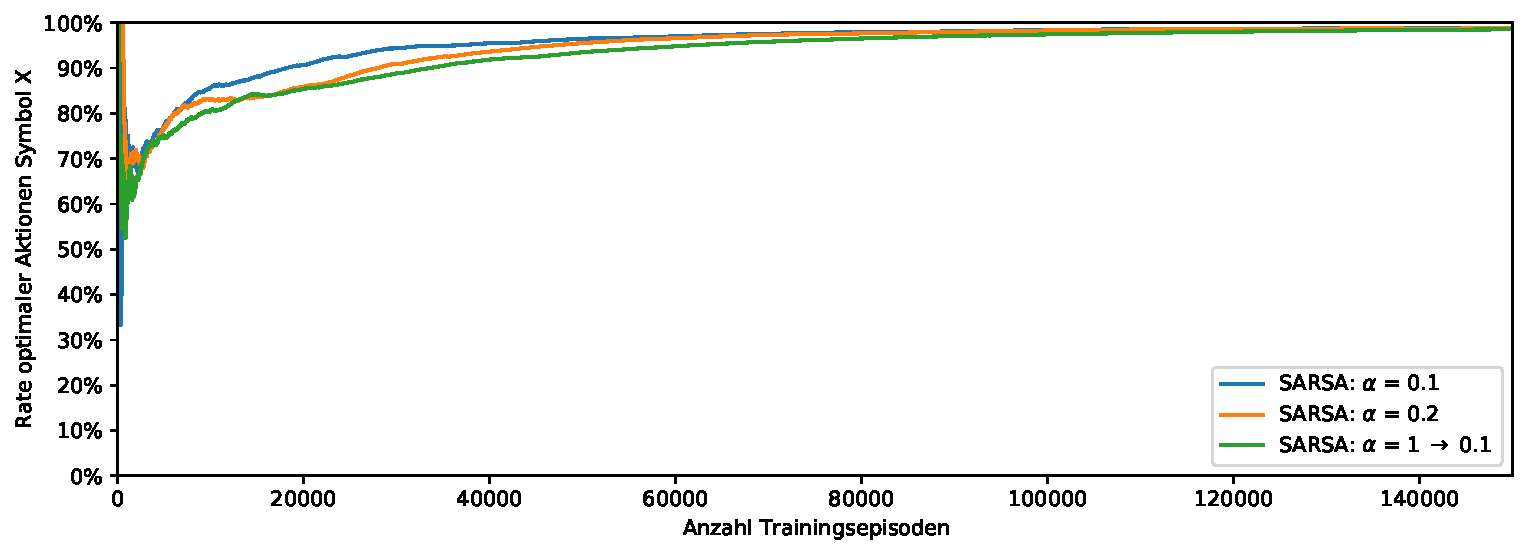
\includegraphics[width=1\linewidth]{convergence/convergence_compare_alpha_SARSA_ALTERNATE_X.pdf}
   \caption{Symbol X}
   \label{fig:convergence_compare_alpha_SARSA_ALTERNATE_X} 
\end{subfigure}

\begin{subfigure}[b]{0.75\textwidth}
    \centering
   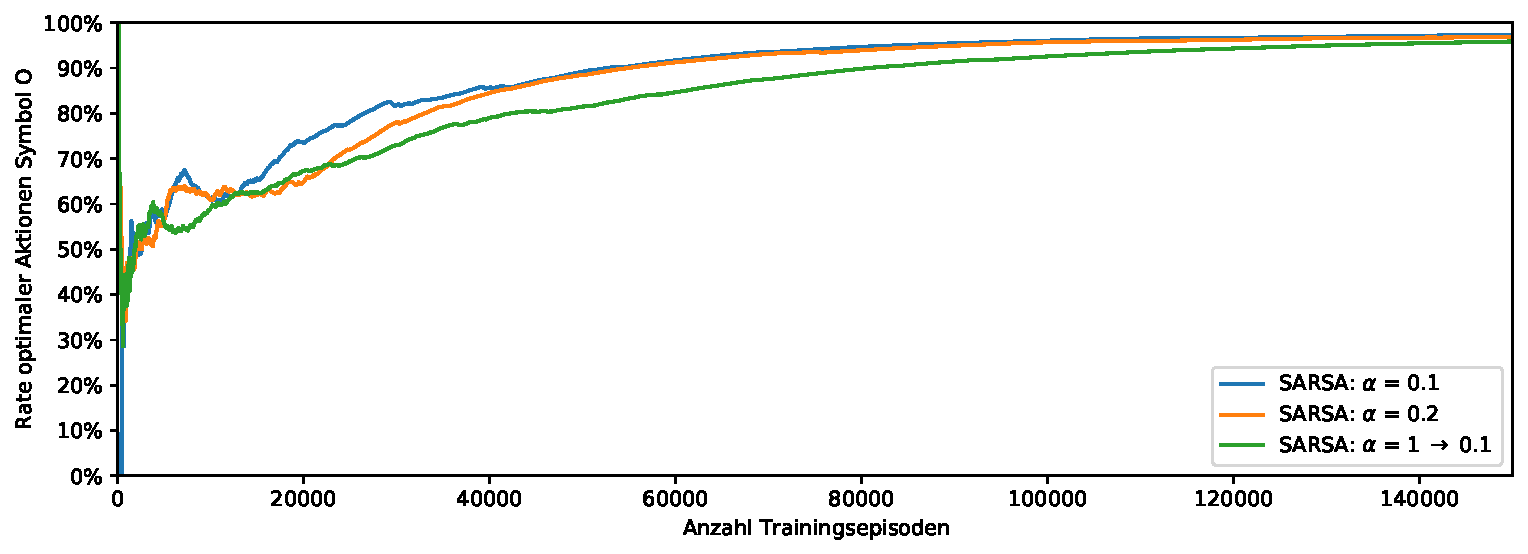
\includegraphics[width=1\linewidth]{convergence/convergence_compare_alpha_SARSA_ALTERNATE_O.pdf}
   \caption{Sybmol O}
   \label{fig:convergence_compare_alpha_SARSA_ALTERNATE_O}
\end{subfigure}

\caption[Rate optimaler Aktionen \sarsa unterschiedliche Lernraten, alternierendes \splay]{Rate optimaler Aktionen von \sarsa für verschiedene Lernraten $\alpha$, alternierendes \splay (a) Symbol X (b) Symbol O}
\label{fig:convergence_compare_alpha_SARSA_ALTERNATE}
\end{figure}

\section{Spielergebnismatritzen klassisches Self-play}
\begin{table}
\centering
\caption[Spielergebnismatrix \sarsa: $\alpha=0,2$, klassisches \splay]{Spielergebnismatrix für \sarsa mit Lernrate $\alpha=0,2$, klassisches \splay}
%\label{tab:resultmatrix_sarsa_normal_alpha02}

\begin{tabular}{llrlr}
\toprule
 & \multicolumn{2}{l}{\textbf{Minimax}} & \multicolumn{2}{l}{\textbf{Random}} \\ \midrule
\textbf{X Sarsa}        & X Sarsa:          & 0,00\% $\pm$    0,00\%            & X Sarsa:              & 98,92\% $\pm$ 0,09\%  \\
                        & O Minimax:        & 0,00\% $\pm$    0,00\%            & O Random:             & 0,00\% $\pm$  0,00\%  \\
                        & Unentschieden:    & 100,00\% $\pm$  0,00\%            & Unentschieden:        & 1,08\% $\pm$  0,09\%  \\ \cmidrule{2-5}
\textbf{O Sarsa}        & X Minimax:        & 0,85\% $\pm$    1,05\%            & X Random:             & 0,18\% $\pm$  0,16\%  \\
                        & O Sarsa:          & 0,00\% $\pm$    0,00\%            & O Sarsa:              & 87,25\% $\pm$ 1,37\%  \\
                        & Unentschieden:    & 99,15\% $\pm$   1,05\%            & Unentschieden:        & 12,57\% $\pm$ 1,21\%  \\ \bottomrule
\end{tabular}
\end{table}
\begin{table}
\centering
\caption[Spielergebnismatrix \sarsa: abnehmende Lernrate, klassisches \splay]{Spielergebnismatrix für \sarsa mit abnehmender Lernrate, klassisches \splay}
%\label{tab:resultmatrix_sarsa_normal_alpha_decay}

\begin{tabular}{llrlr}
\toprule
 & \multicolumn{2}{l}{\textbf{Minimax}} & \multicolumn{2}{l}{\textbf{Random}} \\ \midrule
\textbf{X Sarsa}        & X Sarsa:          & 0,00\% $\pm$    0,00\%            & X Sarsa:              & 98,68\% $\pm$ 0,50\%  \\
                        & O Minimax:        & 0,00\% $\pm$    0,00\%            & O Random:             & 0,00\% $\pm$  0,00\%  \\
                        & Unentschieden:    & 100,00\% $\pm$  0,00\%            & Unentschieden:        & 1,32\% $\pm$  0,50\%  \\ \cmidrule{2-5}
\textbf{O Sarsa}        & X Minimax:        & 0,73\% $\pm$    1,18\%            & X Random:             & 0,14\% $\pm$ 0,18\%  \\
                        & O Sarsa:          & 0,00\% $\pm$    0,00\%            & O Sarsa:              & 87,19\% $\pm$ 2,22\%  \\
                        & Unentschieden:    & 99,27\% $\pm$   1,18\%            & Unentschieden:        & 12,67\% $\pm$ 2,12\%  \\ \bottomrule
\end{tabular}
\end{table}

\section{Spielergebnismatritzen alternierendes Self-play}

\begin{table}[!h]
\centering
\caption[Spielergebnismatrix \sarsa: $\alpha=0,1$, alternierendes \splay]{Spielergebnismatrix für \sarsa mit Lernrate $\alpha=0,1$, alternierendes \splay}
%\label{tab:resultmatrix_sarsa_alternate_alpha01}

\begin{tabular}{llrlr}
\toprule
 & \multicolumn{2}{l}{\textbf{Minimax}} & \multicolumn{2}{l}{\textbf{Random}} \\ \midrule
\textbf{X Sarsa}        & X Sarsa:          & 0,00\% $\pm$    0,00\%            & X Sarsa:              & 95,97\% $\pm$ 2,93\%  \\
                        & O Minimax:        & 8,81\% $\pm$    15,25\%           & O Random:             & 1,38\% $\pm$  2,02\%  \\
                        & Unentschieden:    & 91,19\% $\pm$   15,25\%           & Unentschieden:        & 2,65\% $\pm$  1,03\%  \\ \cmidrule{2-5}
\textbf{O Sarsa}        & X Minimax:        & 3,29\% $\pm$    4,41\%            & X Random:             & 2,48\% $\pm$  0,51\%  \\
                        & O Sarsa:          & 0,00\% $\pm$    0,00\%            & O Sarsa:              & 84,36\% $\pm$ 1,09\%  \\
                        & Unentschieden:    & 96,71\% $\pm$   4,41\%            & Unentschieden:        & 13,15\% $\pm$ 0,96\%  \\ \bottomrule
\end{tabular}
\end{table}
\begin{table}[!h]
\centering
\caption[Spielergebnismatrix \sarsa: $\alpha=0,2$, alternierendes \splay]{Spielergebnismatrix für \sarsa mit Lernrate $\alpha=0,2$, alternierendes \splay}
%\label{tab:resultmatrix_sarsa_alternate_alpha02}

\begin{tabular}{llrlr}
\toprule
 & \multicolumn{2}{l}{\textbf{Minimax}} & \multicolumn{2}{l}{\textbf{Random}} \\ \midrule
\textbf{X Sarsa}        & X Sarsa:          & 0,00\% $\pm$    0,00\%            & X Sarsa:              & 97,15\% $\pm$ 1,42\%  \\
                        & O Minimax:        & 0,00\% $\pm$    0,00\%            & O Random:             & 0,60\% $\pm$  0,63\%  \\
                        & Unentschieden:    & 100,00\% $\pm$  0,00\%            & Unentschieden:        & 2,25\% $\pm$  0,84\%  \\ \cmidrule{2-5}
\textbf{O Sarsa}        & X Minimax:        & 3,29\% $\pm$    4,17\%            & X Random:             & 1,54\% $\pm$  0,62\%  \\
                        & O Sarsa:          & 0,00\% $\pm$    0,00\%            & O Sarsa:              & 85,22\% $\pm$ 1,19\%  \\
                        & Unentschieden:    & 96,71\% $\pm$   4,17\%            & Unentschieden:        & 13,24\% $\pm$ 1,19\%  \\ \bottomrule
\end{tabular}
\end{table}
\begin{table}[!t]
\centering
\caption[Spielergebnismatrix \sarsa: abnehmende Lernrate, alternierendes \splay]{Spielergebnismatrix für \sarsa mit abnehmender Lernrate, alternierendes \splay}
%\label{tab:resultmatrix_sarsa_alternate_alpha_decay}

\begin{tabular}{llrlr}
\toprule
 & \multicolumn{2}{l}{\textbf{Minimax}} & \multicolumn{2}{l}{\textbf{Random}} \\ \midrule
\textbf{X Sarsa}        & X Sarsa:          & 0,00\% $\pm$    0,00\%            & X Sarsa:              & 98,80\% $\pm$ 0,10\%  \\
                        & O Minimax:        & 0,00\% $\pm$    0,00\%            & O Random:             & 0,00\% $\pm$  0,00\%  \\
                        & Unentschieden:    & 100,00\% $\pm$  0,00\%            & Unentschieden:        & 1,20\% $\pm$  0,10\%  \\ \cmidrule{2-5}
\textbf{O Sarsa}        & X Minimax:        & 0,00\% $\pm$    0,00\%            & X Random:             & 0,38\% $\pm$  0,20\%  \\
                        & O Sarsa:          & 0,00\% $\pm$    0,00\%            & O Sarsa:              & 86,83\% $\pm$ 0,54\%  \\
                        & Unentschieden:    & 100,00\% $\pm$  0,00\%            & Unentschieden:        & 12,79\% $\pm$ 0,37\%  \\ \bottomrule
\end{tabular}
\end{table}